\label{sec:kd_susy_smita}
The heavy mass of the top quark could lead to its supersymmetric partner being the lightest squark. PI De's group has been searching for the stop in \D0\ and ATLAS since the discovery of the top quark. So far, this has led to multiple successful Ph.D. thesis from both Tevatron and LHC data -- but alas no sign of the stop. De's latest student, Smita Darmora, defended her Ph.D. thesis on the search for the stop in August, 2015. Her work was co-supervised by base funded researcher Guilio Usai. The title of her thesis was: ``Search for a Supersymmetric Partner to the Top Quark using Multivariate Analysis Technique.'' 

\begin{figure}[hbt]
\begin{center}
  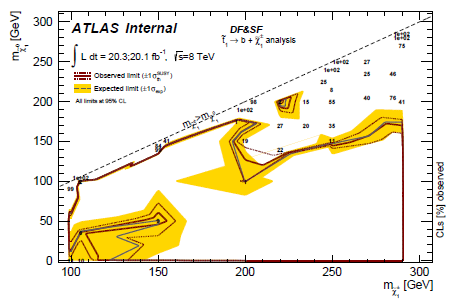
\includegraphics[width=5in]{De/smita_limit.png}
  \caption{Exclusion limit for a 300 GeV mass stop obtained by combining MET trigger and Lepton trigger samples from a Ph.D.  thesis written by Smita Darmora.}
  \label{smita_limit}
\end{center}
\end{figure}

Smita's search focussed on the decay of the stop quark to a chargino and a bottom quark. The chargino subsequently decays to a lepton and missing Et (which comes from the missing neutrino and the missing LSP). The final state is then missing Et with two opposite sign leptons and two b-jets. The primary backgrounds to this channel are top pair production, di-boson production and Z plus jets. The compressed mass spectrum from the chargino-neutralino mass difference leads to soft leptons among the decay products, making this search challenging. We optimized the search separately for soft leptons and hard leptons. Initially, Smita tried a cut based analysis. To improve on the results obtained from the cut based analysis, a multivariate analysis was attempted. This led to a significant increase in the search sensitivity.

The multivariate analysis (MVA) technique used for this search employed a ``supervised learning'' algorithm. A Boosted Decision Tree (BDT) technique was used with a Gradient boosting algorithm, commonly known as BDTG. The TMVA training used eleven classifiers. In rank of importance, missing Et, ratio of leptonic and jet Pt's, and angle between lepton and missing Et had the highest importance. Ten of the chosen variables had non-zero significance. After a long and complicated analysis, 
Figure~\ref{smita_limit} shows the 95\% confidence limit exclusion limit for a 300 GEV mass stop obtained by Smita.



The analysis of Run 1 data is completed. We are continuing the search for stop quark pairs produced in final states with two leptons with Run 2 data. At this stage, Jared Little is setting up our code to run with the new derived data format for Run 2. Darmora and Usai are also involved. We are trying to understand the background distributions in Run 2, with it's higher energy and luminosity. Most of the Monte Carlo samples have already been generated. We are setting up a cut based analysis. We expect to complete the cut based analysis in early 2017. Later in 2017, we will train the TMVA analysis. Both the same sign and opposite sign lepton samples will be analyzed. We will also optimize the analysis for soft leptons. We plan to explore more sophisticated Deep Learning techniques to increase the sensitivity of this search. By the end of 2018, we will be ready to do the analysis with 100 fb$^{-1}$ of data. By the spring or summer of 2019, we will present the results with this large data sample. Finally, in 2020 we will conclude this search with the full Run 2 data sample.
